\documentclass[11pt]{beamer}
\usetheme{Warsaw}
\usepackage[T1]{fontenc}
%\usepackage[utf8]{inputenc}
\usepackage{amsmath}
\usepackage{amsfonts}
\usepackage{amssymb}
\usepackage{graphicx}
\graphicspath{{imgs/}}
\usepackage{setspace}
\usepackage{hyperref}
\usepackage{listings}
\usepackage{xcolor}
%\usepackage{minted}


\author{Chen Zhang \inst{1,2}}
\title{Slide Template}
\setbeamertemplate{enumerate items}[default]


\logo{
\includegraphics[width=.25\textwidth]{logo.jpg}}

\institute[UNI]{\inst{1}Institute 1, \inst{2}Institute 2 $@$ Shenzhen, China\\[2.5ex] {Git URL: \href{https://github.com/CubicZebra/}{\color{cyan}\underline{CubicZebra}}}}

\date{}

% customized
\newcommand{\code}[1]{\texttt{#1}}
\AtEndDocument{\begin{frame}{\huge \quad The End.}\end{frame}}

\definecolor{comment}{rgb}{0, 0.6, 0}
\definecolor{keyword}{rgb}{0.96, 0.52, 0.02}
\definecolor{string}{rgb}{0.12, 0.4, 0.87}
\definecolor{background}{rgb}{0.95,0.95,0.92}
\lstdefinestyle{mypython}{
	language=Python,
    backgroundcolor=\color{background},   
    commentstyle=\color{comment},
    keywordstyle=\color{keyword},
    numberstyle=\tiny\color{magenta},
    stringstyle=\color{string},
    basicstyle=\ttfamily\footnotesize,
    breakatwhitespace=false,         
    breaklines=true,                 
    captionpos=b,
    keepspaces=true,
    numbers=left,
    numbersep=5pt,
	showspaces=false,
	showstringspaces=false,
    showtabs=false,
    tabsize=2
}
\lstset{style=mypython}


\begin{document}

\begin{frame}
\titlepage
\end{frame}

\begin{frame}
\tableofcontents
\end{frame}

\section{Section 1}
\subsection{subsection 1.1}
\begin{frame}{items and code}
\begin{enumerate}
	\item text item 1:
		\begin{enumerate}
			\item something about item 1
			\item another thing about item 1
		\end{enumerate}
    \item code item 2:
    \begin{enumerate}
		\item can use code like: \code{conda activate env}
		\item or multi-lines: \\
		\code{for s in "Hello World":}\\
		\qquad \code{print(s)}
	\end{enumerate}
\end{enumerate}
\end{frame}

\subsection{subsection 1.2}
\begin{frame}{layout and style}
    \begin{minipage}[t]{0.5\textwidth}
        \vspace{0pt}
        \begin{itemize}
            \item emphasis \emph{one} and \emph{two}
            \item customize via \emph{\color{red}three} syntax
            \item code \code{rm} is dangerous $\rightarrow$ \\ {\footnotesize\color{olive}(*more flexible \code{customize} and figure insert)}
        \end{itemize}
    \end{minipage}%
    \hfill
    \begin{minipage}[t]{0.45\textwidth}
        \vspace{0pt}
        \centering
        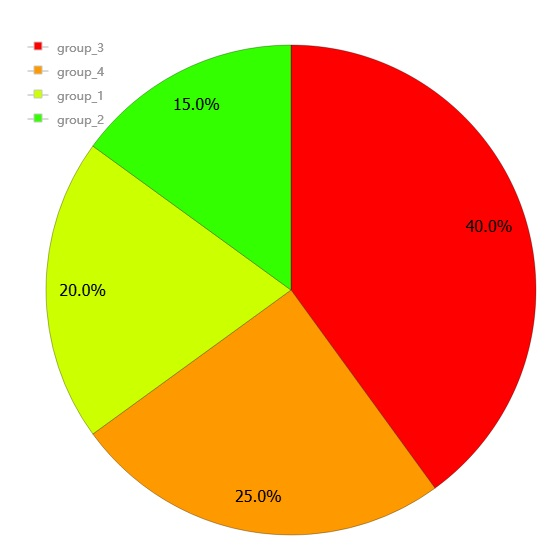
\includegraphics[height=2.5cm, width=2.5cm]{fig1.jpg}
    \end{minipage}
\end{frame}

\section{Section 2}
\subsection{subsection 2.1}
\begin{frame}[t]{another layout}
	\begin{minipage}[t]{1\textwidth}
        \vspace{0pt}
        \begin{itemize}
            \item {try vertical layout like:}\\
            \singlespacing
            \centering
            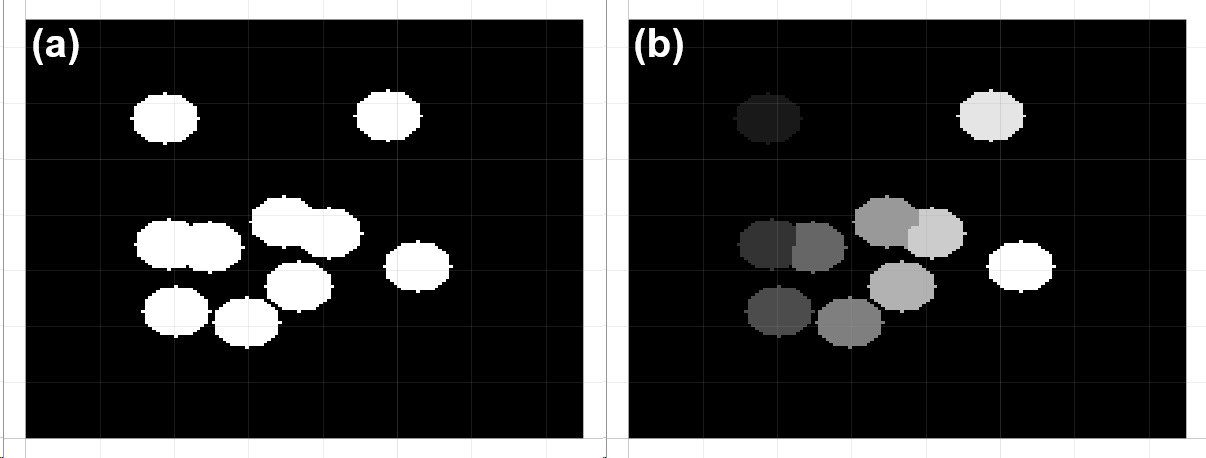
\includegraphics[scale=0.5]{fig2.jpg}
        \end{itemize}
    \end{minipage}%
\end{frame}


\subsection{subsection 2.2}
\begin{frame}{some math expression}
	\begin{enumerate}
		\item for plain: \\ $\because m \in (0, 1] \therefore \eta = 2m/(1+m) \in (0, 1]$
		\item for bold: \\ $\boldsymbol{X} = \boldsymbol{uu}^T$
	\end{enumerate}
\end{frame}

\subsection{subsection 2.3}
\begin{frame}{code snippet}
	\begin{minipage}[t]{0.5\textwidth}
		import from whole script like:
		\lstinputlisting[language=Python]{beamer.py}
    \end{minipage}%
    \hfill
    \begin{minipage}[t]{0.45\textwidth}
    		or for specified snippet, with caption:
    		\lstinputlisting[language=Python, caption=list comprehension, firstline=4,lastline=6]{beamer.py}
    \end{minipage}
\end{frame}

\end{document}